\documentclass[draftclsnofoot,10pt,onecolumn]{IEEEtran} %!PN

\usepackage[margin=0.5cm]{caption}
\usepackage{lipsum}

\usepackage{graphicx}   
\usepackage[export]{adjustbox} 
\usepackage{epstopdf}

\usepackage[justification=centering]{caption}

\usepackage{amssymb}                                         
\usepackage{amsmath}                                         
\usepackage{amsthm}                                          

\usepackage{alltt}                                           
\usepackage{float}
\usepackage{color}

\usepackage{hyperref}
\usepackage{url}

\usepackage{array}

\usepackage{balance}
\usepackage[TABBOTCAP, tight]{subfigure}
\usepackage{enumitem}

\newcommand{\ignore}[2]{\hspace{0in}#2} %Used for inline comments
\newcommand{\tab}{\hspace*{2em}} %For tabbing

\usepackage{pstricks, pst-node}

\usepackage{geometry}
%\usepackage{graphicx}
\geometry{textheight=10in, textwidth=7.5in, margin=0.75in}

\usepackage{listings}

\definecolor{mygreen}{rgb}{0,0.6,0}
\definecolor{mygray}{rgb}{0.5,0.5,0.5}
\definecolor{mymauve}{rgb}{0.58,0,0.82}
\linespread{1}

\lstset{ %
  basicstyle=\ttfamily,            % the size of the fonts that are used for the code
  breakatwhitespace=false,         % sets if automatic breaks should only happen at whitespace
  breaklines=true,                 % sets automatic line breaking
  captionpos=b,                    % sets the caption-position to bottom
  commentstyle=\color{mygreen},    % comment style
  escapeinside={\%*}{*)},          % if you want to add LaTeX within your code
  extendedchars=true,              % lets you use non-ASCII characters; for 8-bits encodings only, does not work with UTF-8
  keepspaces=true,                 % keeps spaces in text, useful for keeping indentation of code (possibly needs columns=flexible)
  keywordstyle=\color{blue},       % keyword style
  %numbers=left,                    % where to put the line-numbers; possible values are (none, left, right)
  %numbersep=10pt,                  % how far the line-numbers are from the code
  %numberstyle=\tiny\color{mygray}, % the style that is used for the line-numbers
  rulecolor=\color{black},         % if not set, the frame-color may be changed on line-breaks within not-black text (e.g. comments (green here))
  showspaces=false,                % show spaces everywhere adding particular underscores; it overrides 'showstringspaces'
  showstringspaces=false,          % underline spaces within strings only
  showtabs=false,                  % show tabs within strings adding particular underscores
  stepnumber=1,                    % the step between two line-numbers. If it's 1, each line will be numbered
  stringstyle=\color{mymauve},     % string literal style
  tabsize=8,                       % sets default tabsize to 8 spaces
  %title=\lstname                  % show the filename of files included with \lstinputlisting; also try caption instead of title
}

\lstdefinelanguage{JavaScript}{
  morekeywords={var, function},
  morecomment=[s]{/*}{*/},%
  morecomment=[l]//,%
  morestring=[b]",%
  morestring=[b]'%
}

\usepackage{hyperref}

\def\BibTeX{{\rm B\kern-.05em{\sc i\kern-.025em b}\kern-.08em
    T\kern-.1667em\lower.7ex\hbox{E}\kern-.125emX}}
    
%\usepackage{floatrow}
\usepackage{lipsum}

    
\renewcommand{\lstlistingname}{Code Snippet:}


\begin{document}
% Hide page numbers
\pagenumbering{gobble}

%\title{Using the Style File IEEEtran.sty} 
\title{Tools for Supporting Community Growth in Open Source \\ {\large CS462: Midterm Report Spring 2016}}

\author{Bruntmyer J. Author, OSU, Goossens M. Author, OSU, Nguyen H. Author, OSU}

%\markboth{Tools for Supporting Community Growth in Open Source}
%{Murray and Balemi: Using the style file IEEEtran.sty} %!PN
%{Murray and Balemi: Using the Document Class IEEEtran.cls} %!PN


\maketitle
%\thispagestyle{plain}\pagestyle{plain}
\begin{abstract}
For the past six months our group has been working on a project that is creating tools that
gives users the ability to look for open source community leaders that are
hosting events about projects that they are leading. These tools will allow
users to have the opportunity to find these events in order to become a
contributor to an open source project. This is done in a form of a website that
will have features for finding certain events dealing with open source projects
so that it can be easily accessible by people with a passion for wanting to
contribute to projects. Throughout this document, we look at what this team has
accomplished for each of the requirements we have laid out, discussing problems
that have halted our progression through the project, and what we have left to
do before completion of the project. We are currently at a strong beta level
stage for this project as we continue to develop for our version 1.0
release. Also included are important images of the user interface we have decided
to use, along with pieces of code that we have completed and worked with thus
far. By the end of this document, you will get a complete picture of how we
reached our beta level tools and what we have left to finish before we have
a version 1.0 ready to be distributed.
\end{abstract}

\newpage

\pagenumbering{arabic}

\section{PROJECT PURPOSES AND GOALS}
After continuous work on this project, the perspective on what
this community development tool wants to accomplish became clear. After taking
more time to read and understand the code that was previously written for the
prototype, we can see clearly on how exactly the data is organized and connected
using Django and its tools. First and foremost, the purpose of the community
development tool remains the same. The purpose is to gather information from
meetup.com and parse that information into a list of upcoming events related to
Apache and open source projects so that developers in the open source community
have an easy way to access an environment where they can hope to participate in those
events.

\section{CURRENT PROGRESSION THROUGH REQUIREMENTS}

\subsection{Fix the People page where the list of community leaders are shown}
\begin{enumerate}[label*=\arabic*.]
  \item Completed Implementation: The “People” page currently takes all of the
    people in the database and lists them onto the page. Normally, if the
    prototype is hosted on a local machine and the database is relatively small,
    then the page loads fine in a minimal amount of time. The issue is nested in
    the actual hosted site by Apache where hundreds of thousands people are
    imported into the database daily and dramatically slowing down the loading
    time of the page.  With our current progression of the project, we have not
    made significant progress into improving the loading time of the page. We
    use our own local host to import a small amount of members at a time and
    that requirement is set to be worked on shortly for Beta implementation. The
    guideline for working towards accomplishing this requirement is to limit the
    amount of people loaded at a time onto the page. For Beta, we have
    rearranged where the table is generated for the people page in the function
    within views.py. This change specifically was introduced because a bug was
    found where when the table is generated, then if the amount of people were
    too many, then the table would crash and not build. With the rearrangement,
    now the table does not break through a large build and now tends to load
    faster. Unfortunately, the implementation of the fix for the People page is
    local. We have yet to test it on the host that Apache is using to run the
    prototype currently. We predict that the fix will work but it will need to
    be approved and patched into the live site for clarification.
\end{enumerate}

\begin{figure}[H]
  \begin{center}
	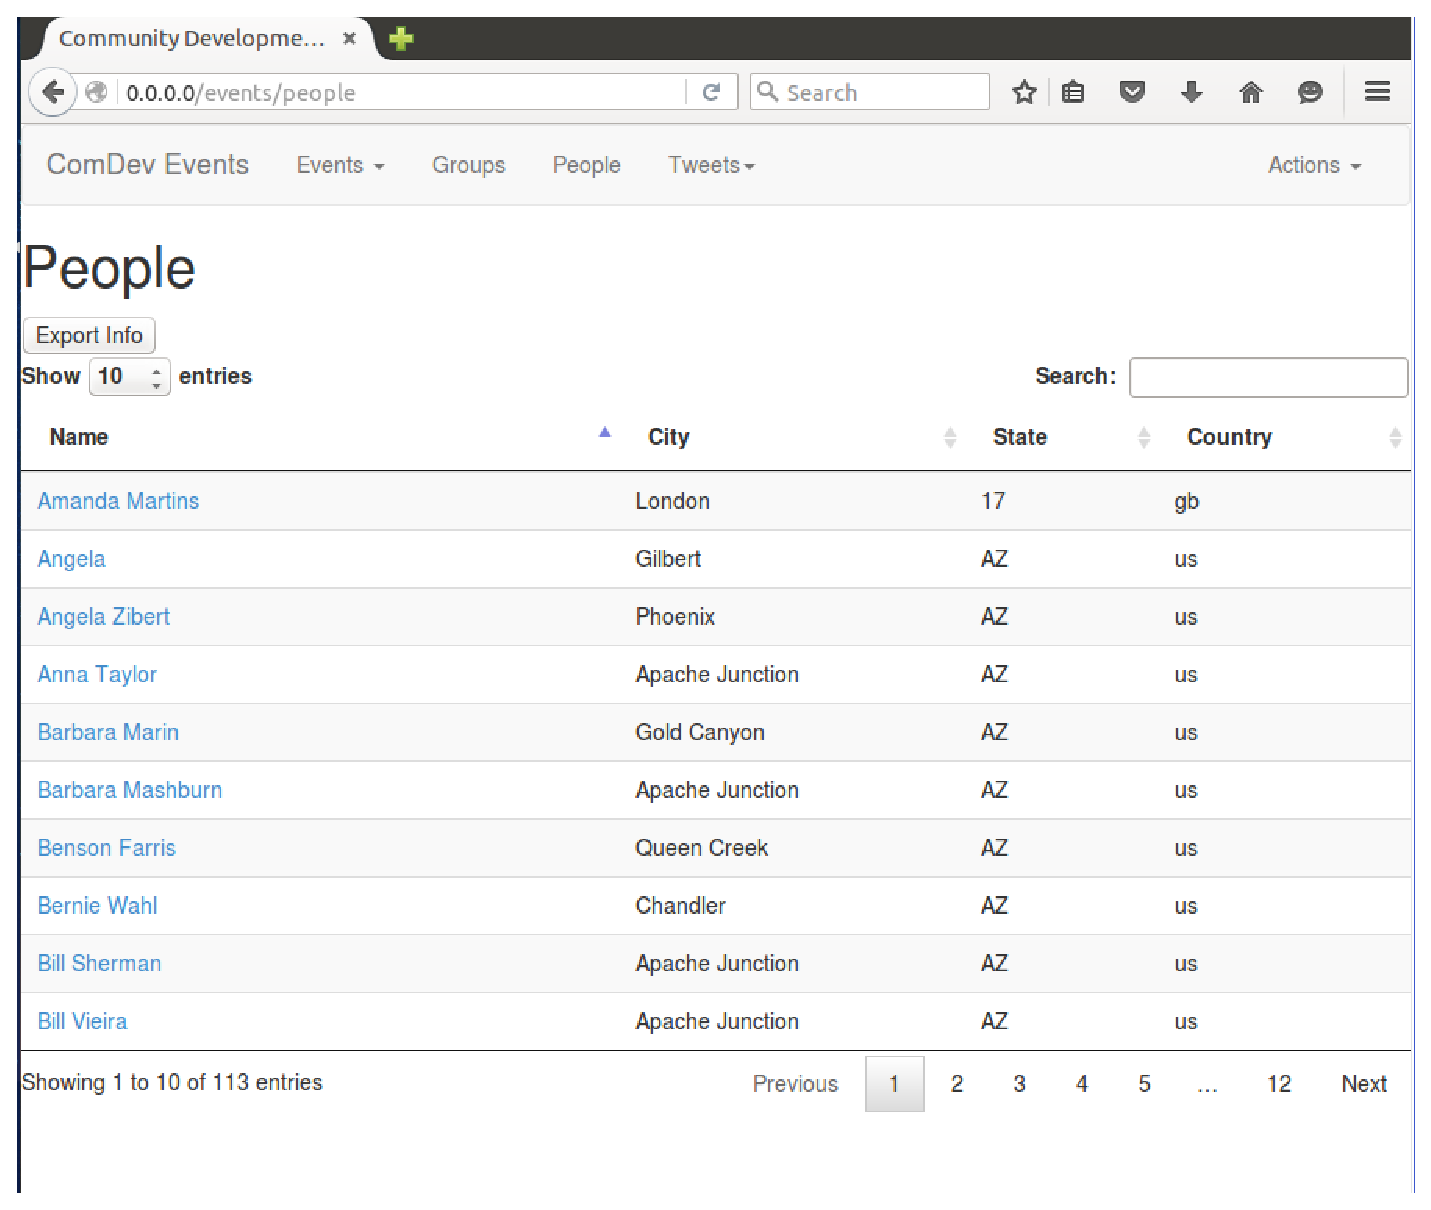
\includegraphics[width=5in, frame]{peoplePage}
	\captionsetup{width=.4\linewidth}
	\centering
  \caption{The people page displaying the profile links for the people that have been imported into the application.}
  \end{center}
\end{figure}

\subsection{Tweet at a person listed in the database}
\begin{enumerate}[label*=\arabic*.]
  \item Current Progress: Currently, a person is generated their own profile page
    based off of their Meetups ID and information from meetups about the person’s
    profile is also parsed in the community development tool. Now those profiles
    include displaying the twitter handle of the person. This was done by changing
    the Meetup API URL request so that we could get the correct information and
    then storing that information in our database. This can be seen in code snippet 1 located below with the URL shown along with the 'if' statements to locate the twitter handle. This allows the user to
    identify a way to get in contact with the person in the profile. Above the
    twitter handle is a button that has the Twitter symbol which allows the user
    to click and send a tweet at the person via Hoot-suite. The hoot-suite app is
    given the twitter handle of the person the user wants to tweet at and the URL
    of the persons page on our application for reference. The user signs in to
    compose the tweet and sends it successfully. The code snippet 2 located below shows the HTML encoding of the button used to create the Hootsuite connection and shows the retrieval of the twitter handle form the database with 'person.service'.

  \item Things to Complete: The tweeting button we have implemented currently
    shows up on a persons profile even if they do not have a twitter handle
    registered with the Meetup website thus having no purpose. To complete this
    requirement completely we would like to hide that button from the user when
    a person does not have a twitter handle registered.
      
%\end{enumerate}

%Below is views.py for showing how the twitter handle is obtained and stored
\begin{center}
  \captionsetup{width=.5\linewidth}
  \begin{lstlisting}[caption=Views.py file where twitter handle is identified and stored, language=Python]
            url = "https://api.meetup.com/2/members?offset=0&format=json&group_id=" + 
            str(group.meetupID) + "&photo-host=public&page=500&sig_id=148657742&key=" + 
            MEETUP_API_KEY
            response = urllib2.urlopen(url)
            result = response.read()

            data = json.loads(result)
            members = data['results']

            for member in members:
                try:
                    person = Person.objects.get(meetupID = member['id'])
                except Person.DoesNotExist:
                    person = Person()

                try:
                    person.meetupID = member['id']
                    person.name = member['name']
                    #person.service = member['other_services']['twitter']['identifier']
                    person.country = member['country']
                    if 'other_services' in member.keys():
                        if 'twitter' in member['other_services'].keys():
                            if 'identifier' in member['other_services']['twitter'].keys():
                                person.service = member['other_services'}
                                                       ['twitter']['identifier']
  \end{lstlisting}
\end{center}
    
%Below is view.html for showing the twitter handle and the button for tweeting
  \begin{center}
  \captionsetup{width=.5\linewidth}
   \begin{lstlisting}[caption=View.py where the button for tweeting at a person is created and twitter handle is displayed., language=HTML]
        <a href="{{ person.service }}" title="{{ person.service }}" 
        		class="_hs_socialshare" > Tweet at this Person </a>
          <script>
            var _hs = {
                       size: 5,
                       partner: "community.apache.org"
            };
            (function() {
                         var h = document.createElement('script'); h.type = 
                         'text/javascript'; h.async = true;
                         h.src = ('https:' == document.location.protocol ? 'https://' : 
                         'http://') + 'dtirydke3kdq7.cloudfront.net/hootlet.js?v=1';
                         var s = document.getElementsByTagName('script')[0]; s.parentNode.insertBefore(h, s);
            })();
          </script>
   \end{lstlisting}
\end{center}

\begin{figure}[H]
  \begin{center}
  
\includegraphics[width=3in, frame]{tweet_person1}
  	\captionsetup{width=.4\linewidth}
  \centering
  \caption{The button that is displayed when a user has a twitter handle that is publicly available on Meetups that allows a user to tweet at the person.}

  \end{center}
\end{figure}

\begin{figure}[H]
  \begin{center}
  
  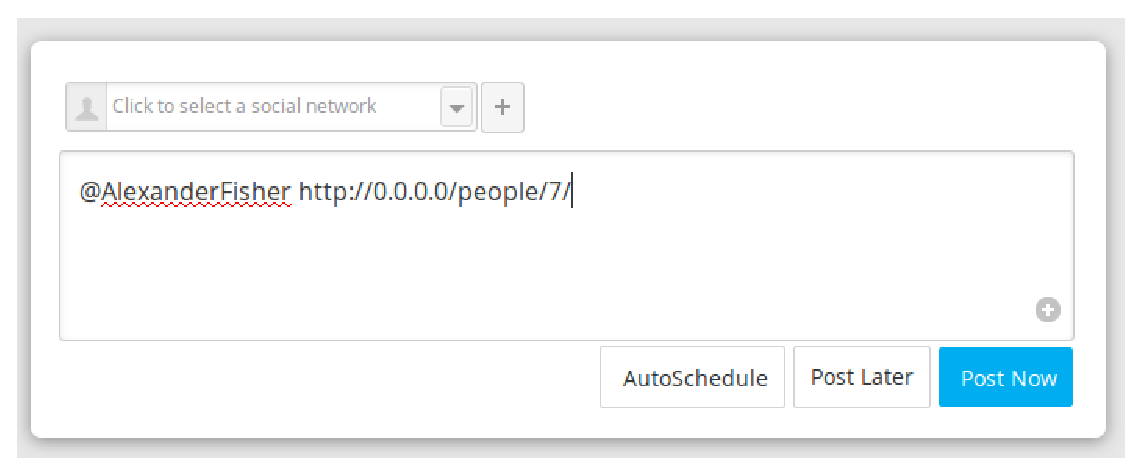
\includegraphics[width=3in, frame]{tweet_person2}
  	\captionsetup{width=.4\linewidth}
  \centering
  \caption{The HootSuite service is used to send the tweet at the person as we supply the twitter handle and it is up to the user to use their Twitter account to tweet.}

  \end{center}
\end{figure}

\end{enumerate}

\subsection{Add user accounts to application and track when a user has tweeted an event}
\begin{enumerate}[label*=\arabic*.]
  \item Completed Implementation: The purpose of adding user accounts to the applications
    is to be able to track when users tweeting about events or people. With the completion
    of this requirement, the account creation is working along with being able to sign in 
    successfully with a confirmation of signing in by displaying a welcome message along with
    the user's username. There is also a login and logout button located in the
    top right section of the website on all pages allowing the user to login or
    logout at anytime. Everything is also backended with features of the website only existing
    if the user has an authorized account. This means that action functions within the application
    which include importing meetups, importing members, marking events as not
    applicable, and marking groups as not applicable to be behind being signed in.
    This means if you are not logged in with the authorized account, you can't perform these 
    actions. Note that the accounts created are allowed access to these features, but do not
    have access to the administrative page that deals with the Django database.

\end{enumerate}
\begin{center}
\captionsetup{width=.5\linewidth}
  \begin{lstlisting}[caption=Views.py file that handles the creation of accounts and the login page view, language=Python]
        def login(request):
            state = "Please log in below..."
            username = password = ''
            if request.POST:
                username = request.POST.get('username')
                password = request.POST.get('password')

                user = authenticate(username=username, password=password)
                if user is not None:
                    if user.is_active:
                        auth_login(request, user)
                        state = "Welcome " + username + "!"
                    else:
                        state = "Your account is not active, please contact the site admin."
                else:
                    state = "Your username and/or password were incorrect."
            template = loader.get_template('login/login.html')
            context = RequestContext(request, {
                                     'state': state,
                                     'username': username
            })
            return HttpResponse(template.render(context))

        def logout_view(request):
            logout(request)
            return render(request, 'login/login.html')

        def createAccount(request):
            if request.POST:
                username = request.POST.get('username')
                password = request.POST.get('password')
                email = request.POST.get('email')
                first_name = request.POST.get('first_name')
                last_name = request.POST.get('last_name')

                user = User.objects.create_user(username, email, password)
            return render(request, 'login/createAccount.html')
      \end{lstlisting}
    \end{center}

    \begin{center}
    \captionsetup{width=.5\linewidth}
        \begin{lstlisting}[caption=urls.py file where the destinations are stored for login and logout, language=Python]
          url(r'^accounts/login/$', views.login, name='login'),
          url(r'^logout', views.logout_view, name='logout'),
          url(r'^login/$', views.login, name='login'),
          url(r'^createAccount/$', views.createAccount,  name='createAccount'),
          url(r'^index/$', views.index, name='eventIndex'),
      \end{lstlisting}
    \end{center}

\begin{figure}[H]
  \begin{center}
  
  
\includegraphics[width=3in, frame]{createAccountForm}
  \captionsetup{width=.4\linewidth}
  \centering
  \caption{Example usage of the create account form. }

  \end{center}
\end{figure}

\begin{figure}[H]
  \begin{center}
  
  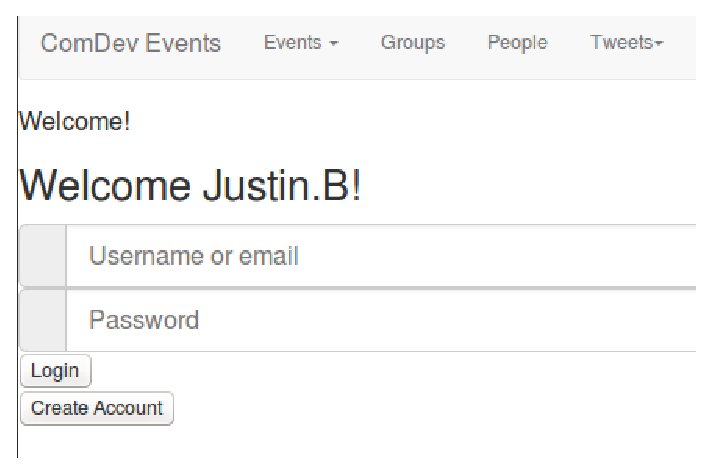
\includegraphics[width=3in, frame]{loginSuccess}
  \captionsetup{width=.4\linewidth}
  \centering
  \caption{Showing created user actually signing into the website. }

  \end{center}
\end{figure}

\subsection{List tweets about events and/or people via the application}
\begin{enumerate}[label*=\arabic*.]
  \item Completed Implementation: We were unable to track the precise tweets
    made from our application, but we have found an alternative that mostly
    works. As shown in the code snippet, the website makes a call to Twitter's
    search API, requesting all tweets that contain a certain hashtag as well as
    the hashtag \#Meetup. The hashtags are the same as the ones used to get
    events from meetup.com. Once it has the tweets, it uses the id from each one
    to make another call to Twitter's OEmbed API, which sends back HTML that is
    used in the page's template to present embedded tweets to users. This still
    pulls a few tweets that are unrelated, but bit of filtering would work.
    Unfortunately this would be difficult, and is outside the scope of our
    project.
\end{enumerate}

\begin{center}
\captionsetup{width=.5\linewidth}
  \begin{lstlisting}[caption=Views.py showing the Twitter authorization and
  search for tweets from the application., language=Python]
    def _twitterAuth():
        # Encode the keys
        key = base64.b64encode(TWITTER_API_KEY)

        # Set needed values
        authURL = "https://api.twitter.com/oauth2/token"
        content_type = "application/x-www-form-urlencoded;charset=UTF-8"
        body = "grant_type=client_credentials"

        # Create the header
        authHeaders = {'Content-Type': content_type, 'Authorization': "Basic " + key}
        # Get auth
        auth = requests.post(authURL, headers=authHeaders, data=body)
        # Get the response in a useable format
        authJSON = auth.json()
        
        return authJSON['access_token']

    def _oembedTweets(tweets):
        hashtags = Hashtag.objects.all().exclude(name = "Meetup")
        oembed = dict()
        for hashtag in hashtags:
            oembed[hashtag.name] = []
            for i in range(0, len(tweets[hashtag.name]) - 1):
                url = "https://api.twitter.com/1/statuses/oembed.json?id=" + str(tweets[hashtag.name][i])
                embededResponse = requests.get(url)
                embeded = embededResponse.json()
                oembed[hashtag.name].append(embeded['html'])

        return oembed

    def tweetsApp(request):
        # Auth with Twitter
        accessToken = _twitterAuth()

        # Get hashtags
        hashtags = Hashtag.objects.all().exclude(name = "Meetup")

        oembed = []
        allTweets = dict()
        for hashtag in hashtags:
            allTweets[hashtag.name] = []
            url = "https://api.twitter.com/1.1/search/tweets.json?q=%23" + hashtag.name + "+%23Meetup&src=typd"
            headers = {'Authorization': "Bearer " + accessToken}
            response = requests.get(url, headers=headers)
            tweetsJSON = response.json()
            for tweet in tweetsJSON['statuses']:
                allTweets[hashtag.name].append(tweet['id'])

        oembed = _oembedTweets(allTweets)

        return render(request, 'tweets/app.html', {'tweets': oembed})
  \end{lstlisting}
\end{center}

\subsection{List tweets about events and/or people not via the application}
\begin{enumerate}[label*=\arabic*.]
  \item Completed Implementation: The website now has a tweet parser. As shown
    in the code snippet, it sends a call to Twitter's search API, requesting all
    tweets with a certain hashtag. The hashtags are the same as the ones used to
    get events from meetup.com. Once it has the tweets, it uses the id from each
    one to make another call to Twitter's OEmbed API, which sends back HTML that
    is used in the page's template to present embedded tweets to users.  The
    search results currently contain all instances of the hashtag requested,
    even when they are not relevant to any event, or even open source. The
    search needs refinement, however, this will be difficult, and is not within
    the scope of the project
\end{enumerate}

\begin{center}
\captionsetup{width=.5\linewidth}
  \begin{lstlisting}[caption=Views.py showing the Twitter authorization and
  searching for tweets for the tweets not from the application, language=Python]
    def _twitterAuth():
        # Encode the keys
        key = base64.b64encode(TWITTER_API_KEY)

        # Set needed values
        authURL = "https://api.twitter.com/oauth2/token"
        content_type = "application/x-www-form-urlencoded;charset=UTF-8"
        body = "grant_type=client_credentials"

        # Create the header
        authHeaders = {'Content-Type': content_type, 'Authorization': "Basic " + key}
        # Get auth
        auth = requests.post(authURL, headers=authHeaders, data=body)
        # Get the response in a useable format
        authJSON = auth.json()
        
        return authJSON['access_token']

    def _oembedTweets(tweets):
        hashtags = Hashtag.objects.all().exclude(name = "Meetup")
        oembed = dict()
        for hashtag in hashtags:
            oembed[hashtag.name] = []
            for i in range(0, len(tweets[hashtag.name]) - 1):
                url = "https://api.twitter.com/1/statuses/oembed.json?id=" + str(tweets[hashtag.name][i])
                embededResponse = requests.get(url)
                embeded = embededResponse.json()
                oembed[hashtag.name].append(embeded['html'])

        return oembed

    def tweetsNotApp(request):
        # Auth with twitter
        accessToken = _twitterAuth()

        # Get the hashtags
        hashtags = Hashtag.objects.all().exclude(name = "Meetup")

        allTweets = dict()
        for hashtag in hashtags:
            allTweets[hashtag.name] = []
            url = "https://api.twitter.com/1.1/search/tweets.json?q=%23" + hashtag.name + "&src=typd"
            headers = {'Authorization': "Bearer " + accessToken}
            response = requests.get(url, headers=headers)
            tweetsJSON = response.json()
            for tweet in tweetsJSON['statuses']:
                allTweets[hashtag.name].append(tweet['id'])

        oembed = _oembedTweets(allTweets)

        return render(request, 'tweets/notApp.html', {'tweets': oembed})
  \end{lstlisting}
\end{center}

\begin{figure}[H]
  \begin{center}
  
  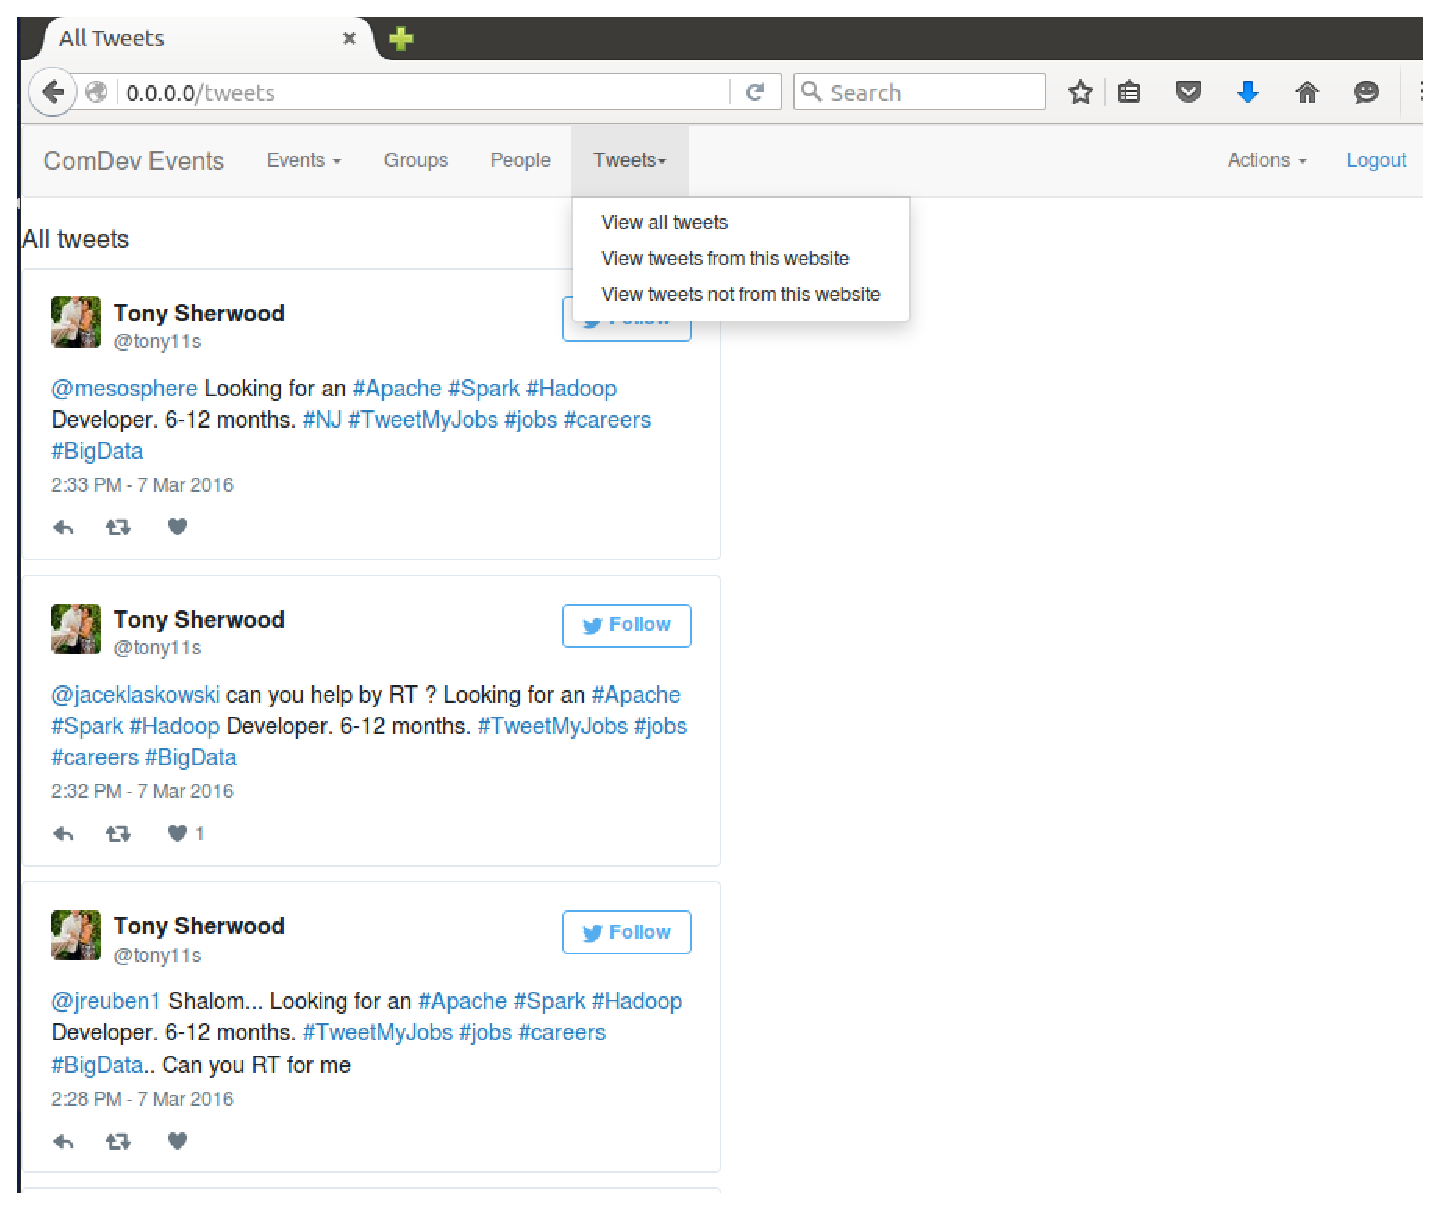
\includegraphics[width=5in, frame]{listingTweets}
  \captionsetup{width=.4\linewidth}
  \centering
  \caption{Showing our application listing the tweets that are located on twitter. }

  \end{center}
\end{figure}

\subsection{Export a list of people with Information}
\begin{enumerate}[label*=\arabic*.]
  \item Completed Implementation: When taking on this requirement we quickly realized that
    the Meetup API would not provide email address for its users which was
    understandable. We then looked at what other information would be useful to
    extract about the people that were loaded into the database. This lead us to
    export information such as name, twitter handle, bio, Meetup ID, URL, country,
    state, and city. The export can be executed by clicking on the 'Export Info'
    button located in the top left of the people page and creates a file in a XLSX
    format which can be directly opened or saved.
    
    \begin{center}
    \captionsetup{width=.5\linewidth}
      \begin{lstlisting}[caption=excelutils.py file where the worksheet is generated and exported as an xlsx file, language=Python]
        def WriteToExcel(person_list):
            output = StringIO.StringIO()
            workbook = xlsxwriter.Workbook(output)
            worksheet_s = workbook.add_worksheet("People")

            #write title
            person_text = ugettext("everyone")
            title_text = u"{0} {1}".format(ugettext("Information for"), person_text)
            #merge cells
            worksheet_s.merge_range('B2:I2', title_text, title)

            #write header
            worksheet_s.write(4, 0, ugettext("No"), header)
            worksheet_s.write(4, 1, ugettext("Name"), header)
            worksheet_s.write(4, 2, ugettext("Service"), header)
            worksheet_s.write(4, 3, ugettext("Bio"), header)
            worksheet_s.write(4, 4, ugettext("Country"), header)
            worksheet_s.write(4, 5, ugettext("State"), header)
            worksheet_s.write(4, 6, ugettext("City"), header)
            worksheet_s.write(4, 7, ugettext("MeetupID"), header)
            worksheet_s.write(4, 8, ugettext("URL"), header)

            #column widths
            bio_col_width = 25

            #add data to the table
            for idx, data in enumerate(person_list):
                row = 5 + idx
                worksheet_s.write_number(row, 0, idx + 1, cell_center)
                worksheet_s.write_string(row, 1, data.name, cell)
                worksheet_s.write_string(row, 2, data.service, cell)
                worksheet_s.write_string(row, 3, data.bio, cell)
                worksheet_s.write_string(row, 4, data.country, cell)
                worksheet_s.write_string(row, 5, data.state, cell)
                worksheet_s.write_string(row, 6, data.city, cell)
                worksheet_s.write_number(row, 7, data.meetupID, cell)
                worksheet_s.write_string(row, 8, data.url, cell)

            workbook.close()
            xlsx_data = output.getvalue()           #xlsx_data contains the Excel file
            return xlsx_data
      \end{lstlisting}
    \end{center}
\end{enumerate}


\begin{figure}[H]
  \begin{center}
  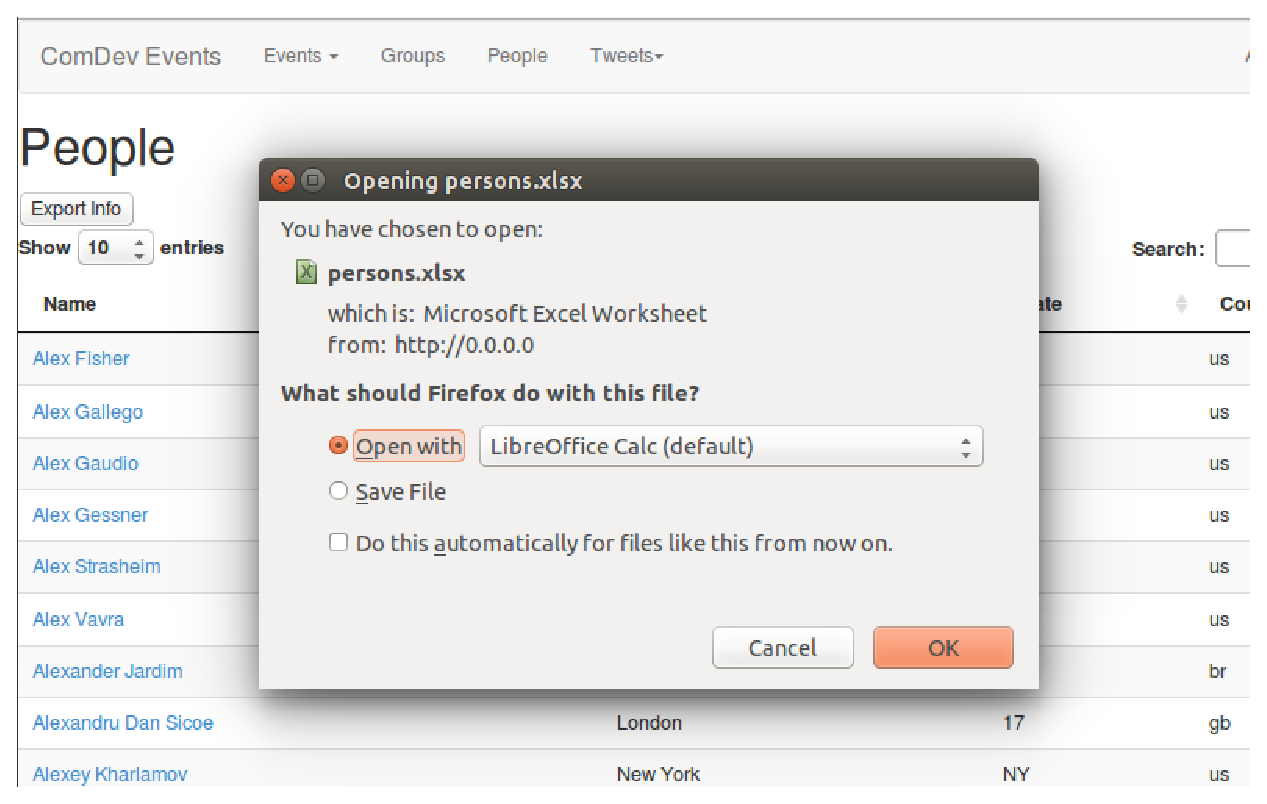
\includegraphics[width=5in, frame]{exporting1}
  \captionsetup{width=.4\linewidth}
  \centering
  \caption{Showing export button executing. }

  \end{center}
\end{figure}

\begin{figure}[H]
  \begin{center}
  
  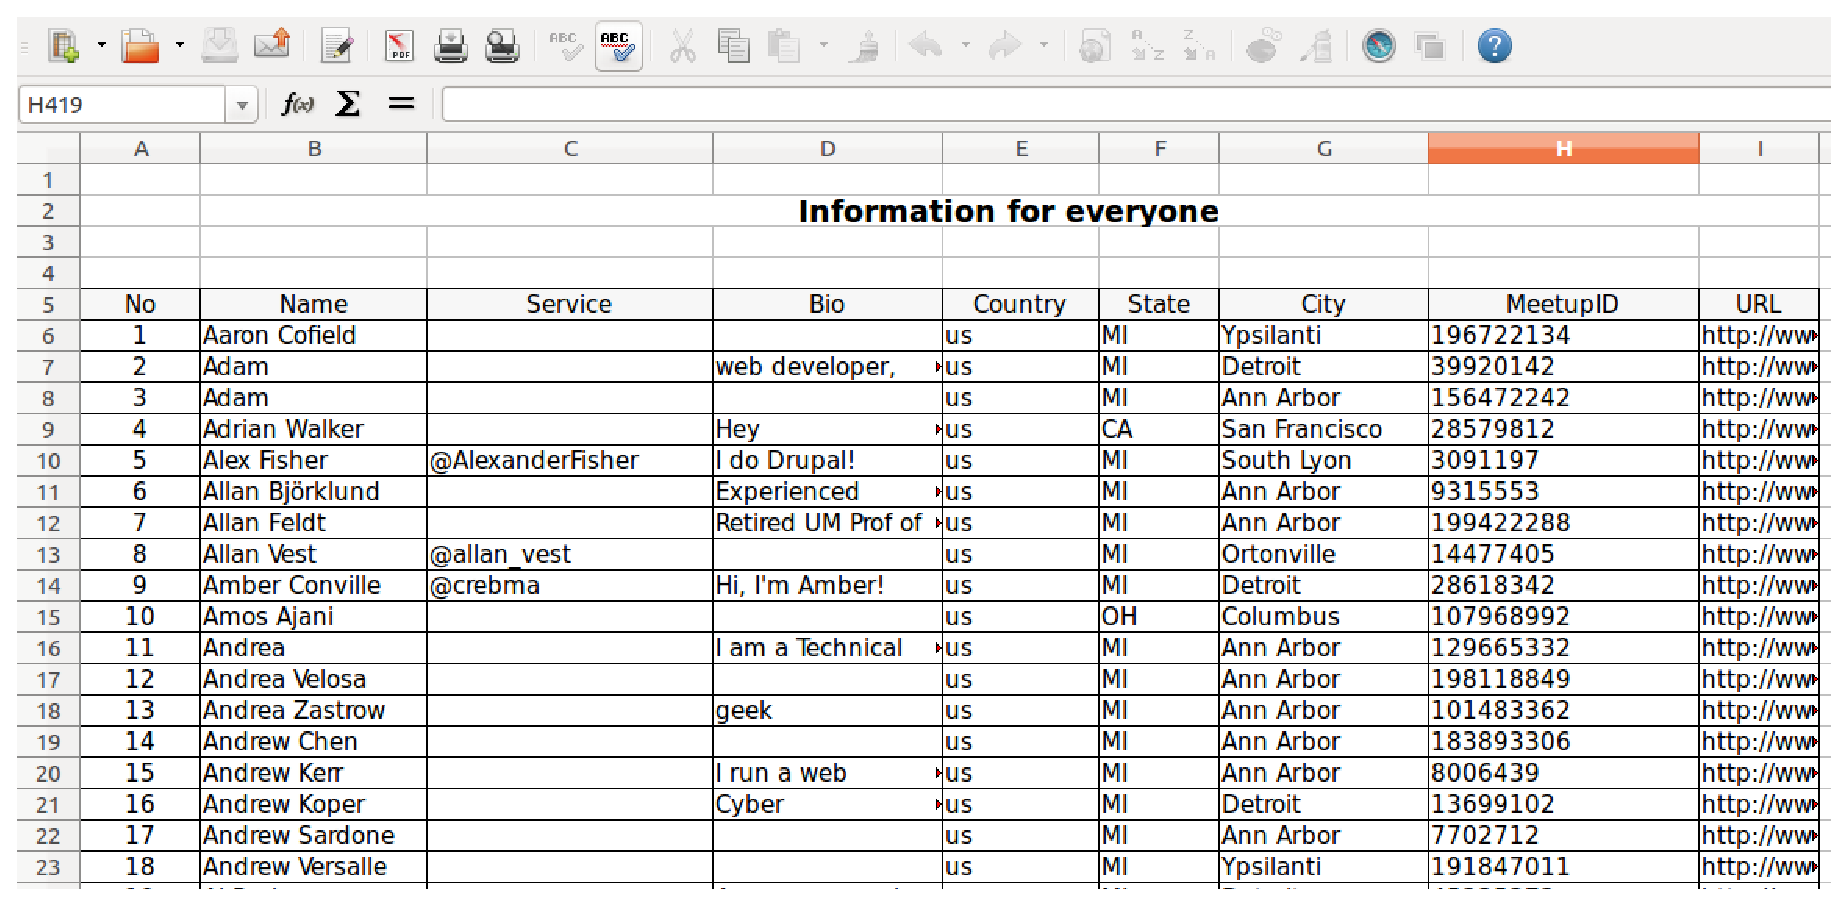
\includegraphics[width=6in, frame]{exporting2}
  \captionsetup{width=.4\linewidth}
  \centering
  \caption{Showing the list of exported information about people that were imported. }

  \end{center}
\end{figure}

\subsection{Improve hashtag searching of application to improve finding more relevant events}
\begin{enumerate}[label*=\arabic*.]
  \item Completed Implementation: The solution to this issue was to change one word in
    the call to the meetup.com API. In the API there are many different
    restrictions you can use to request events. Two of them come into play here:
    "text" and "topic." The text query searches through the content of the
    events, while the topic query looks at the topics related to the group. The
    original query was looking at text, which resulted in a lot of unrelated
    events. The query was fixed to use "topic," which has reduced unwanted events
    significantly. A thourough examination of events imported resulted in no
    unrelated events pulled in.
\end{enumerate}

\subsection{Improve the visuals of the tool's look as a whole}
\begin{enumerate}[label*=\arabic*.]
  \item Completed Implementation: The application itself began as a fairly organized
  	piece. The navigation bar implementation really helps the user keep track navigating
  	between each page. When viewing the list of events, the events are listed in
  	chronological order starting with the most recent. There is a search bar
  	available for the user to type in for a certain event that they wish to view. There
  	are other sorting mechanisms to view those events in another sorting order.
  	Our focus in this requirement were to mainly to improve how data is displayed. This
  	specifically applies to to the event page and people profiles. Along with the addition
  	of the Host objects, the generated host profiles would have a visual update as well.
  	As displayed in Figure 9, the improvement of the profile page is shown with categories
  	specifically labeled and displayed in concrete areas of the page. If the certain variable
  	does not exist, then the user can clearly see where that detail would go on the page.
  	Topics are more clearly organized have are configured under a scrollable table as well.
  	Overall, this addition makes the people profile page much more organized and legible.
  	In addition to the updated people profile page, the event page is also upgraded in Figure
  	10. Similar to the profile upgrade, the event page now has categories that specifically
  	detail where objects belong. This is much more particularly important where the description
  	is displayed for the event. Previously, it was much more difficult for the user's eye to
  	view where the venue of event would be. Now in this update, that portion is clearly labeled
  	which allows the user to spend less time reading and to quickly see the information
  	that they want to. \\
    
\begin{figure}[H]
  \begin{center}
  
  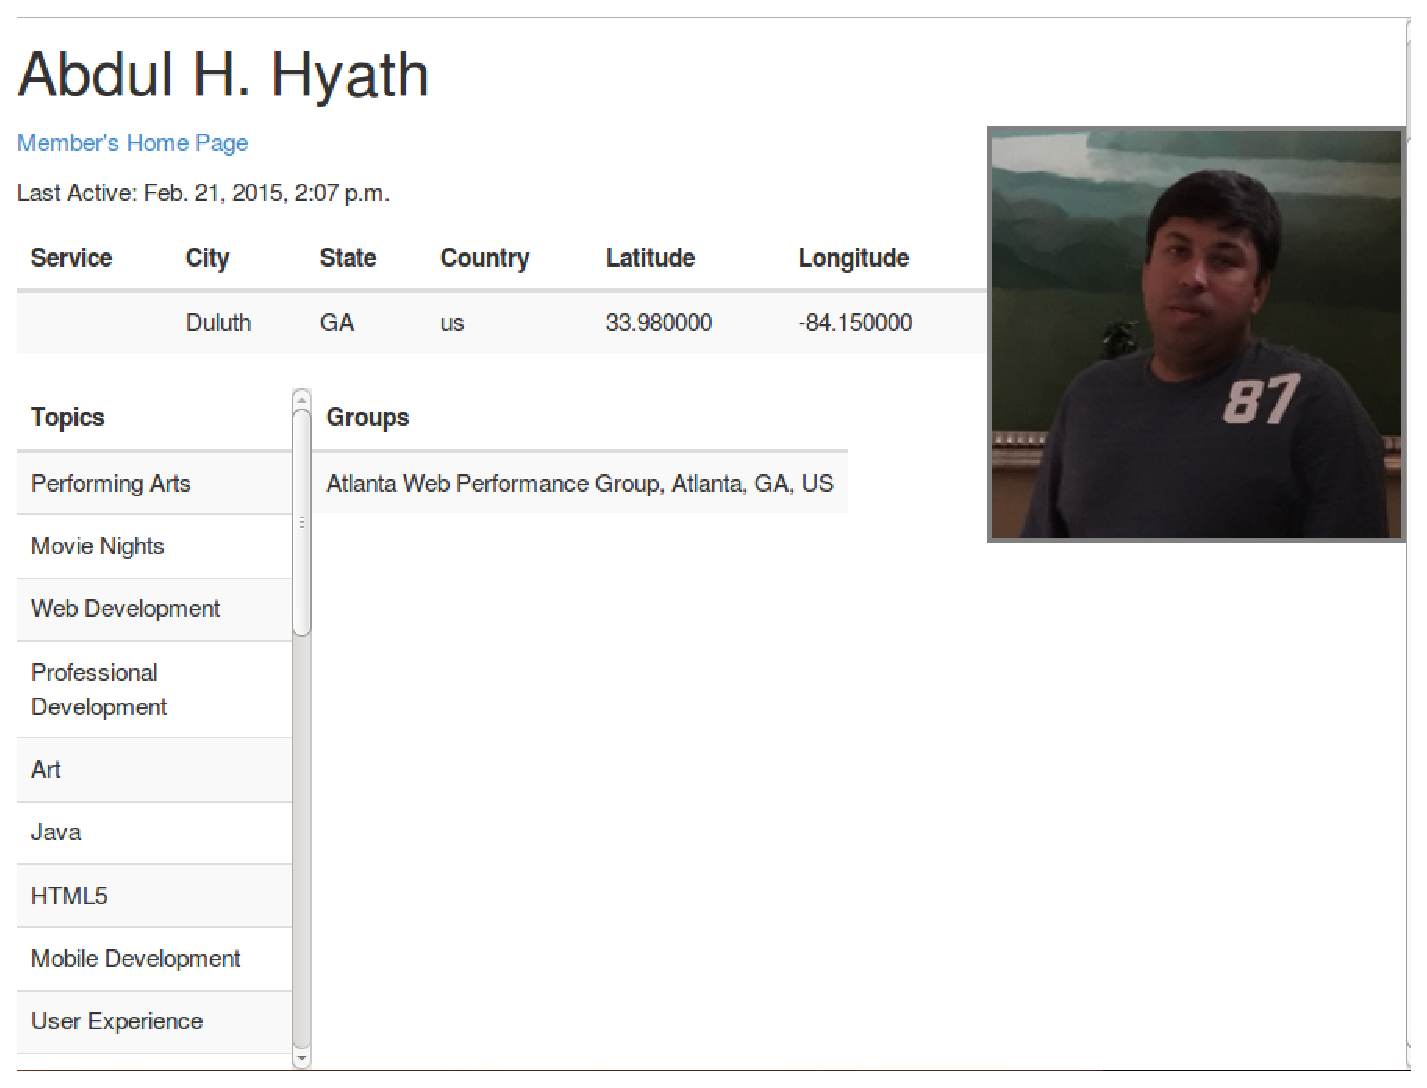
\includegraphics[width=5in, frame]{peopleProfileAfter}
  \captionsetup{width=.4\linewidth}
  \centering
  \caption{Showing updated generated profile for person with 
  organized attributes and scrollable text }
  \end{center}
\end{figure}

\begin{figure}[H]
  \begin{center}
  
  \includegraphics[width=5in, frame]{eventPageAfter}
  \captionsetup{width=.4\linewidth}
  \centering
  \caption{Updated event page with description labels and reorganized arrangements
  with details}
  \end{center}
\end{figure}

    Upon improving the visuals of the website we will want to get feedback on the changes we have 
    made to figure out if those changes have appealed to users of the tool. In order to figure this	
    out we have decided to create a user study where we sit the user down with our website and ask 
    them to complete a list of tasks. We will be interacting with the user and helping them if they 
    have any questions and we will be taking notes as well during the experience.
    Once the set of tasks are attempted or completed we will then have a set of questions that we 
    will ask the user. The list of tasks and questions are shown below: \\

\begin{enumerate}
	\item Tasks:
	\begin{enumerate}
		\item Look through all pages and play with the navigation.
		\item Create an account and login.
		\item Import upcoming open source events.
		\item Import members/hosts of a group.
		\item Browse 2-3 people profiles.
		\item Browse 3-4 groups.
		\item Tweet about an event.
		\item Tweet at a person from the website.
		\item Look for events based on location.
		\item View tweets that are on twitter on the website.
		\item Export some information about people in groups.
		\item Logout. \\
	\end{enumerate}
	\item Questions:
	\begin{enumerate}
		\item On a scale from 1 to 10 how easy was it to navigate this website? (10
    being very easy, 1 being not easy at all)
  		\item What was the feature you found most useful?
  		\item What was the feature you found least useful?
  		\item Would you use this website in the future (Please explain why or why
    not)?
  		\item Would you recommend this website to a friend or colleague?
  		\item If you could add one feature to this website, what would that feature
    be? Why?
    		\item How do you feel about the overall look of the website?
    		\item What would you change visually in the website? Where? \\
	\end{enumerate}
\end{enumerate}

We decided to go with a questionnaire based user study because we feel for functionality it would be great to get feedback on how the user
experiences the tools early on. With the scale of how easy it was to navigate
the website we will be able to get a sense of how everything flows and if
getting the user to the tool they want to use is happening as smoothly as
possible. When asking about a feature the user liked most and least we can get a
better sense of which tools are actually being utilized in the website to either
build on them or decide they are not useful and how we can improve on them.
Asking if the user would either recommend this website to a friend or if they
will use it themselves in the future gives us great feedback on if the user
generally enjoyed the experience with the tool or if the user had a horrible
time and would not return to use this tool again. The last question about the
user adding a feature for the website gives us great feedback to see if we are
missing something crucial that a lot of people would like to use during their
experience using our tool.
\end{enumerate}

\subsection{Implement system of improved sorting of finding events by nearby location within radius of the user}
\begin{enumerate}[label*=\arabic*.]
  \item Current Progress: The current tool has the function to
    create a list of all events parsed through the application and the ability to
    search for a specific event by sorting or an individual search. An additional
    option is added for the user to be able to locate an event based on the
    location that they input within a certain mile radius of that location. The
    current implementation is nearly complete as we are using the Google Maps API
    to display a map and allow the user to enter a location. Once the user has
    entered a location the map is populated with markers which indicate event
    locations. When these markers are hovered over it will display the name of the
    event. This will allow the user to jump to a location on the map and see if
    the event's are nearby. The event search page also lists all events along with
    latitude, longitude, and start time. When no event's are imported the user can
    still use the map but there will be no markers displayed and the list will
    display the message 'No events available'.

  %\item Current Progress: The current tool has the function to create a list of
    %all events parsed through the application and the ability to search for a
    %specific event by sorting or an individual search. An additional option is
    %added for the user to be able to locate an event based on the location that
    %they input within a certain mile radius of that location. The current
    %implementation of this requirement has the searching bar created, but does
    %not yet have the implementation of the actual searching algorithm ready.

  \item Things to Complete: We will be adding more details to the markers
    themselves which feature a short summary of the event along with the local
    start time displayed both will appear when click on. We would also like to
    have the map be centered on the location of the machine the user is using
    such as taking advantage of location services just for a nice starting
    point. As of right now the centered beginning location is on Corvallis,
    Oregon.

  %\item Things to Complete: Since Apache is open source, some implementation of
    %a searching tool has already been implemented for another project. With
    %that implementation available for reference, the implementation for the
    %application should be in a similar fashion; however, there has been a large
    %issue for this development because the code written is not in the same
    %version of Django as our current application. In addition, trying to
    %understand the implementation for the location services is very difficult
    %to fully comprehend to implement that onto the application. After spending
    %three weeks on trying to implement that portion of the feature, we have not
    %yet been successful and are starting to try to approach this feature in a
    %different method. Django has geo-location services that is actually already
    %in its system, so we are currently looking at that as an alternative
    %option.
%\end{enumerate}

\end{enumerate}

\begin{center}
\captionsetup{width=.5\linewidth}
	\begin{lstlisting}[caption=Views.py shows the eventSearch funciton that allows the view in the template for the events page to pull information from the database. This also shows the URL used to get the info about events along with how it is stored., language=Python]
        def eventSearch(request):
            #return render(request, 'events/eventSearch.html')
            now = datetime.now()
            upcoming_events_list = Event.objects.filter(is_applicable = True).filter(local_start__gte=now).order_by('local_start')
            template = loader.get_template('events/eventSearch.html')
            context = RequestContext(request, {
                                     'upcoming_events_list': upcoming_events_list,
                                     'can_import': _canImport()
            })
            return HttpResponse(template.render(context))
            
        url = "https://api.meetup.com/2/open_events?&sign=true&photo-host=public&state=ky&city=lexington&country=usa&topic=" + hashtag.name + "&radius=10000&sign=true&key=" + MEETUP_API_KEY

         try:
             #getting location of the events instead of groups show below - Justin Bruntmyer
             if 'venue' in meetup.keys():
                 if 'city' in meetup['venue'].keys():
                     event.city = meetup['venue']['city']
                 if 'country' in meetup['venue'].keys():
                     event.country = meetup['venue']['country']
                 if 'state' in meetup['venue'].keys():
                     event.state = meetup['venue']['state']
                 if 'address_1' in meetup['venue'].keys():
                     event.address_1 = meetup['venue']['address_1']
                 if 'lat' in meetup['venue'].keys():
                     event.latitude = meetup['venue']['lat']
                 if 'lon' in meetup['venue'].keys():
                     event.longitude = meetup['venue']['lon']
            #end getting locaiton info - Justin Bruntmyer
	\end{lstlisting}
\end{center}

\begin{center}
\captionsetup{width=.5\linewidth}
	\begin{lstlisting}[caption=The eventSearch.html has a mixture of JavaScript and HTML that create the Google Map and search bar along with creating markers for events., language=JavaScript]
        function initAutocomplete() {
            var map = new google.maps.Map(document.getElementById('map'), {
                center: {lat: 44.5645659, lng: -123.2620435},
                zoom: 13,
                mapTypeId: google.maps.MapTypeId.ROADMAP
            });

            // Create the search box and link it to the UI element.
            var input = document.getElementById('pac-input');
            var searchBox = new google.maps.places.SearchBox(input);
            map.controls[google.maps.ControlPosition.TOP_LEFT].push(input);

            // Bias the SearchBox results towards current map's viewport.
            map.addListener('bounds_changed', function() {
                searchBox.setBounds(map.getBounds());
                });

            var markers = [];
            // Listen for the event fired when the user selects a prediction and retrieve
            // more details for that place.
            searchBox.addListener('places_changed', function() {
                var places = searchBox.getPlaces();

                if (places.length == 0) {
                    return;
                }
                
                //Clear out the old markers.
                markers.forEach(function(marker) {
                    marker.setMap(null);
                });
                markers = [];

                
                    var myLatLng = {lat: {{even.latitude}}, lng: {{even.longitude}}};
                    var marker = new google.maps.Marker({
                        position: myLatLng,
                        map: map,
                        title: '{{ even.name }}'
                    });
                
                // For each place, get the icon, name and location.
                var bounds = new google.maps.LatLngBounds();
                places.forEach(function(place) {
                    var icon = {
                        url: place.icon,
                        size: new google.maps.Size(71, 71),
                        origin: new google.maps.Point(0, 0),
                        anchor: new google.maps.Point(17, 34),
                        scaledSize: new google.maps.Size(25, 25)
                    };

                    // Create a marker for each place.
                    markers.push(new google.maps.Marker({
                        map: map,
                        icon: icon,
                        title: place.name,
                        position: place.geometry.location
                    }));
                    
                    if (place.geometry.viewport) {
                      // Only geocodes have viewport.
                        bounds.union(place.geometry.viewport);
                    } else {
                          bounds.extend(place.geometry.location);
                      }
                  });
                  map.fitBounds(bounds);
                });
         }
	\end{lstlisting}
\end{center}

\begin{figure}[H]
  \begin{center}
  
  \includegraphics[width=5in, frame]{mapSearching}
  \captionsetup{width=.4\linewidth}
  \centering
  \caption{Showing the map of where you can search a location to see nearby events, also listing events locations. }

  \end{center}
\end{figure}

\subsection{Add feature to generate a profile for people and have it display a way to contact the person if a method is available}
\begin{enumerate}[label*=\arabic*.]
  \item Current Progress: The main goal of the tool is to promote community
    development in the open source scene. A very important feature is then to have
    the best information available for users who would like to start development
    to be easily viewable. With a generated profiles for people within active
    groups contributing to Apache projects and project alike that displays a
    method of contacting said person then it will give people a chance to get
    involved with the project. Currently, the people generated profiles show the
    name, a bio, their twitter handle if they have one, location, topics
    interested in, a picture, source linked to profile on meetup.com, last
    activity, and the group they are associated with. Since we are not able to
    pull email address from Meetup we have decided to focus on the service twitter
    handle as a method of contact which is displayed for the user.

  %\item Current Progress: The main goal of the tool is to promote community
    %development in the open source scene. A very important feature is then to
    %have the best information available for users who would like to start
    %development to be easily viewable. With a generated profile for community
    %developers to have their contact information, this eases the process for
    %users in which they can start engaging in the community. Our current
    %implementation with these profiles are the “people” pages in which
    %information about the person is available. Contact information about that
    %specific person is not entirely parsed through and may have to be manually
    %implemented. This part of the feature has been highly discussed within the
    %group as many concerns have come up such as how a user would identify
    %themselves as a community developer or community leader. Permissions that a
    %user would have to add their own events have been discussed but ultimately
    %dismissed because of certain attributes that are undesirable such as

  \item Things to Complete: During the implementation of this requirement we came
    up with the possibility of adding a page just for people who hose events so
    that users can have a chance to contact organizers directly. This will require
    pulling the organizer of each event from the Meetup API, storing it, and
    displaying just as the people page works now. This page will have organizer
    profiles for users to go to.

  %\item Things to Complete: Before fully implementing this system, the issue at
    %the hand is to fully distinguish what part of this development tool will it
    %belong in and who the intended population is. It is important to have
    %community leaders to have their contacting information for the public to see,
    %but it is also dangerous to allow just any individual to post something on an
    %open webpage.
\end{enumerate}

\begin{figure}[H]
  \begin{center}
  
  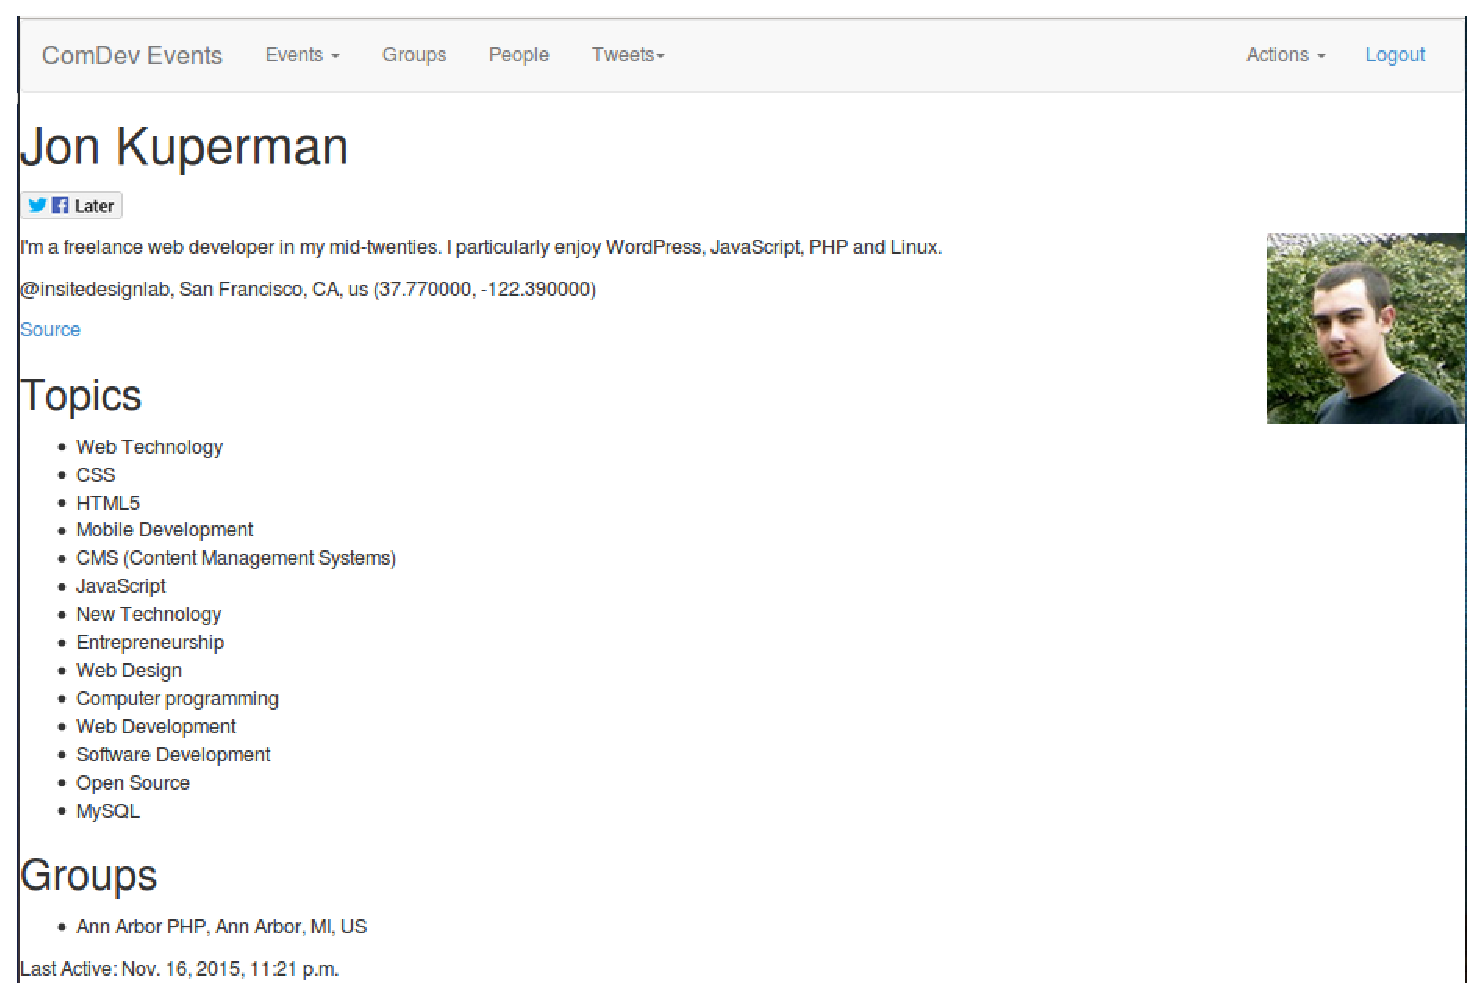
\includegraphics[width=5in, frame]{peopleProfile}
  \captionsetup{width=.4\linewidth}
  \centering
  \caption{Showing profile generated for person along with a twitter handle for a method of contacting. }

  \end{center}
\end{figure}

\section{Feature Requests}
Throughout the presentation of our tools to our client Ross we were happy to hear that he was really excited about the progress we have made thus far.
In his excitement in seeing how far we have come with the tools and the progress he has seen
Ross began asking for feature requests to be added to the tools we have developed thus far.
We decided to add this section to our report so that we could reference Ross's confidence in our team to make these requests possible if we have time.
It is important to note that these requests are in no way suppose to be completed by the end of our time with this project.
These requests are for future ideas for the tools and are options for use to complete if we have time. Our client also would like us to submit patches for the tools
that we have made thus far as he approves of the work we have done. We will be working
on creating these patches in the coming weeks.
The requirements that have had feature requests proposed are shown below.

\subsection{Add user accounts to the application}
\begin{enumerate}
	\item Have a field for the user to enter their Twitter ID if they have one
\end{enumerate}

\subsection{List tweets about events via the app and not via the app}
\begin{enumerate}
	\item Improve quality of what you see currently by caching.
    \item Possibly improve the quality of tweets returned by using Hootsuite.
    \item Search tweets with multiple tags to be displayed.
    \item List all of the users tweets and the ones containing hashtags, separate pages.
    \item Mark users who are in groups that are not relevant just like you can do with the events themselves.
\end{enumerate}

\subsection{Export a list of people with information}
\begin{enumerate}
	\item Add some more fields to the exported list such as what group they are associated with and a list of topics they are interested in.
\end{enumerate}

\subsection{Improve hashtag searching of application for better results on relevant events}
\begin{enumerate}
	\item Find any opportunity to improve the searching by hashtags method. This requirement can always use some tweaking but it is good that the searching has improved.
\end{enumerate}

\subsection{Add feature to generate a profile of people for community developers to have contacting information easily viewable}
\begin{enumerate}
	\item Create profiles for the people that are imported that are hosting the events as these people might be more interesting to contact for community developers.
\end{enumerate}

\subsection{Implement system of improve sorting of finding events by nearby location within radius of the user}
\begin{enumerate}
  \item Have map and list of events and start times be side by side on the page.
  \item Calculate distance from where the user has searched to where the location is and display how far away each location is and sort by distance.
\end{enumerate}

\section{PROBLEMS ENCOUNTERED}

Throughout this term we have encountered many problems that have impeded our
progress for this project. This was to be expected as with all projects. 
Events
occur that can halt progress and bring forth challenges that, as a group, we
needed to overcome. The problems that we have faced are listed below along with
the methods we used to get through the situation. We also ran into the occasioin coding block where we would have days where not much progress was obtained. However, we feel this did not impeded our progress as
it is just part of being a computer scientist.

\subsection{Problem 1}
Deciding which platform we were going to be developing on using Docker. This was
a major issue as we originally planed to work with the Windows operating system
however we could not get the application to run locally on a Windows platform.
We continually ran into errors with creating a local database along with having
the right Docker tools to support the application. We had available resources
such as a README file that gave insight on the problem but whatever we tried did
not seem to work. We eventually shifted gears and decided to try Docker and the
application on Linux, specifically Ubuntu 14.04. Thanks to the Linux knowledge
of Megan Goossens and plenty of online documentation we were able to get Docker
installed successfully along with running the application on a local host. From
this point we decided to continue developing in the Linux environment.

\subsection{Problem 2}
At the end of the Fall 2015 term we set up a weekly meeting with our client
throughout Winter 2016 to discuss implementation details for the week and
planned to utilize this time to make sure everyone is on the same page. Due to
some miss-communication we were unable to meet with our client for the first two
weeks. This halted our progress with because we had a lot of issues with getting
Docker to work with Windows and we were counting on a meeting with our client to
resolves those issues as soon as possible. We eventually got in contact with our
client and figured out what was happening as the first week our client was on an
unexpected trip to the UK and in the second week our client did not realize that
these meetings occurred every week throughout the term. These things happen and
once we all had a chance to get on the same page every weekly meeting is going
smoothly.

\subsection{Problem 3}
During week three of Winter 2016 we ran into the issue of meetings being
canceled due to illness and injury. One of our team members experience an injury
that caused a full group meeting with a TA to occur which halted our progress in
having to get everyone caught up on the same page. This same week another group
member became sick and could not make it to two meetings for the week which
meant that two people could not make it so two meetings were canceled out of the
weekly three meetings we have as a group. This was not too untactful as we were
able to work individually at home but it was still a noticeable disruption from
the normal work we produce in a week. It did not seem like it was going to
effect the group at first however when we began to get back on track it took
some adjustments to makes sure everyone was on the same page and try to make up
for the week we missed.

\subsection{Problem 4}
During the first week of the term we began developing based on the requirements
we had listed in our requirements document. The problem we ran into here was
that we had issues understanding what are requirements were trying to say thus
we went through the document and changed the language used for the requirements.
This did not change the requirement but it made it easier to understand if
someone is reading through it. This took a days worth of progress which was
frustrating due to the fact that we believed to have this done last term. We
currently are happy with the updated requirements document as it has been
approved by our client, professor, and TA. This halted our progress by being an
unnecessary step in the implementation process as it should have been completed
last term.

\section{TIMELINE UPDATE}
When we began the development side of the project we realized that it was best
to strive for achieving alpha level functionality with all of our features that
we would like to have. This required us to take a different approach then what
our timeline originally suggested. With that change we were able to have the
structure ready for us when we began beta level implementation. With all
requirements completed at the beta level we then began to look ahead to see when
we want to accomplish the tiny tweaks and bug fixes for the 1.0 release. \\

We are going to focus our attention on choosing dates to fully implement version 1.0 and 
complete each requirement. This means that we will move on from the expected
completion date for beta to a new date that we will except to have no bugs and tiny
tweaks finished. Below shows our future timeline for getting these items
completed for version 1.0 release. \\

\newcolumntype{C}[1]{>{\centering\let\newline\\\arraybackslash\hspace{0pt}}m{#1}}

\begin{center}
\begin{tabular}{ | C{1cm} | C{7cm}| C{6cm} | } 
\hline
REQ\# & Requirement & Expected Completion (V 1.0) \\ 
\hline
1 & Fix the "People" page where the list of people are shown from groups & Completed \\ 
\hline
2 & Tweet at a person listed in database & Completed \\ 
\hline
3 & Add user accounts to the application and track when a user has tweeted an event & Completed \\ 
\hline
4 & List tweets about events and/or people via the app & Completed \\ 
\hline
5 & List tweets about events and/or people from twitter, but not via the app & Completed \\ 
\hline
6 & Export a list of people with information & Completed \\ 
\hline
7 & Improve hashtag searching of application for better results on relevant events & Completed \\ 
\hline
8 & Implement a system of finding events nearby a location entered or within radius of the user & Completed \\ 
\hline
9 & Add feature to generate a profile for community developers to have contacting information easily visable & Completed \\ 
\hline
10 & Improve the visuals of the tool and how it looks as a whole. & Completed \\ 
\hline
\end{tabular}
\end{center}
\end{document}
